\setcounter{chapter}{0}
\renewcommand{\thechapter}{\Alph{chapter}}
\chapter{Appendices} \label{append}
\section{Neural Network Training for Damage Detection} \label{an:key}

\begin{figure}[H]
	\centering
	\begin{subfigure}{.475\textwidth}
		\centering
		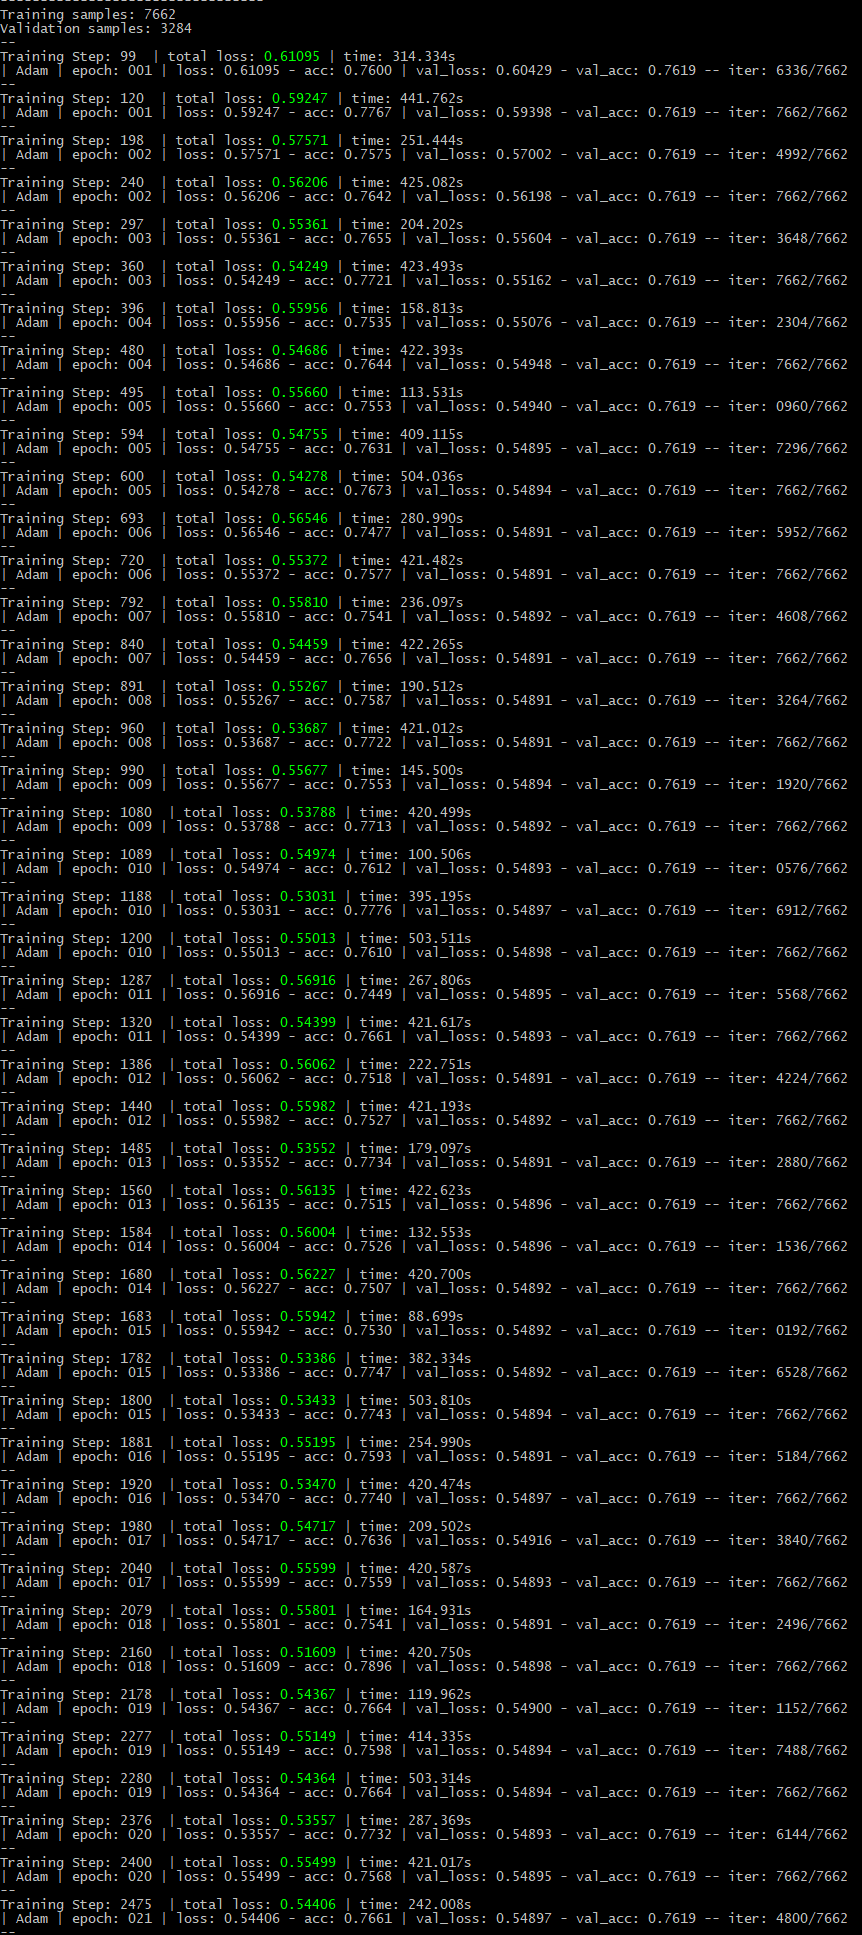
\includegraphics[width=.975\linewidth]{figs/TrainingDet.png}
		\label{fig:NN_R}
	\end{subfigure}
	\begin{subfigure}{.475\textwidth}
		\centering
		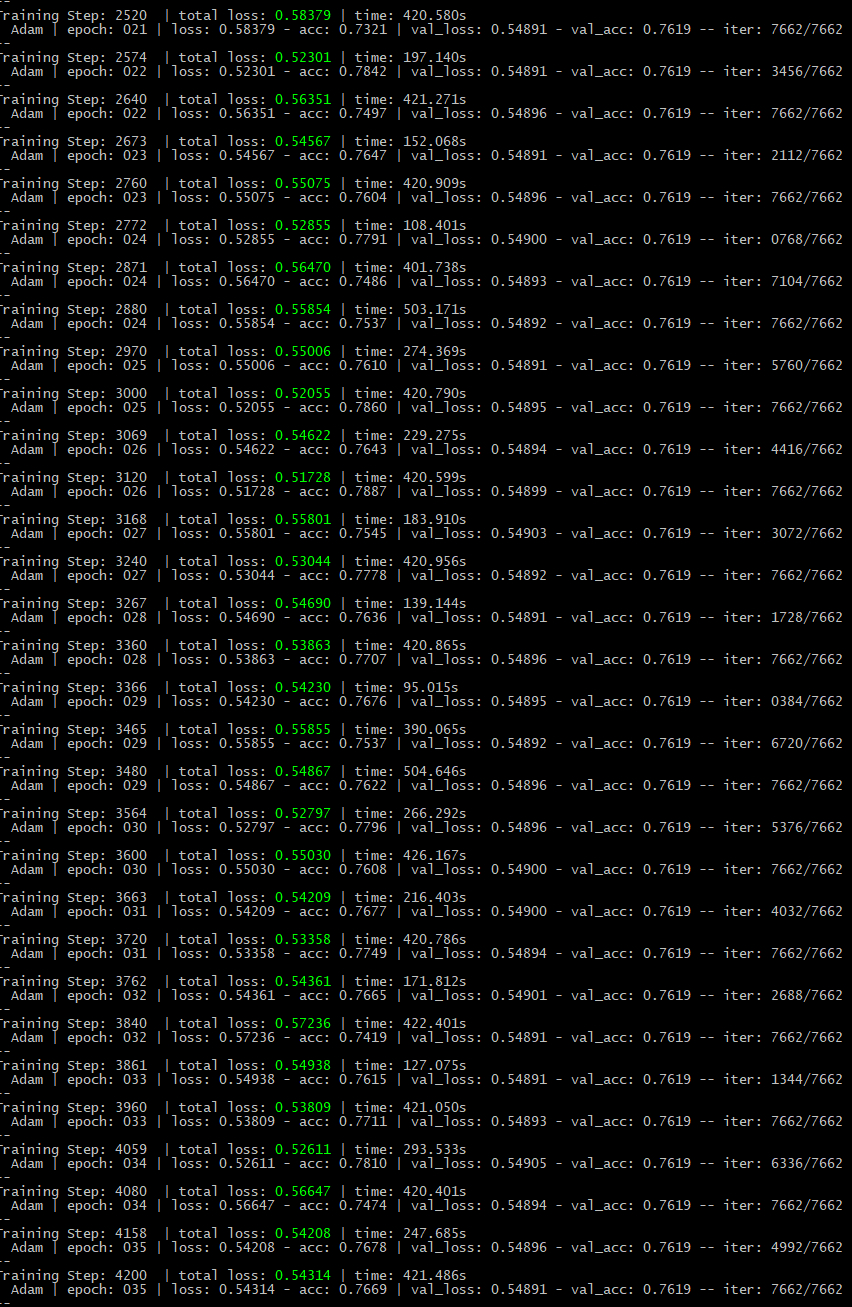
\includegraphics[width=.975\linewidth]{figs/TrainingDet1.png}
		\label{fig:NN_R1}
	\end{subfigure}
	\caption{\footnotesize{Full results training \ac{cnn} with 35 epochs.}}
	\label{fig:an1}
\end{figure}

\section{Results Empirical Approach to Damage Detection} \label{an:coh}

\begin{table} [H]
	\footnotesize
	\captionsetup{justification=raggedright,singlelinecheck=false}
	\caption{Confusion matrix [Vertical Ground Truth, Horizontal predicted] and F1 classification for interferometry univariate change detection with a threshold of 0.30. Cohen Kappa Score: 0.05896}
	\begin{tabular}{l|llll}
		& No    & Damage & unknown &  \\ \hline
		No      & 439.0 & 80.0   & 0.0     &  \\
		Damage  & 254.0 & 67.0   & 0.0     &  \\
		unknown & 12.0  & 4.0    & 0.0     &  \\
		&       &        &         & 
	\end{tabular}
	\begin{tabular}{l|llll}
		& precision & recall & f1-score & support \\ \hline
		No          & 0.44      & 0.21   & 0.28     & 321     \\
		Damage      & 0.62      & 0.85   & 0.72     & 519     \\
		unknown     & 0.00      & 0.00   & 0.00     & 16      \\
		avg / total & 0.54      & 0.59   & 0.54     & 856    
	\end{tabular}

	\label{tab:matInt}
\end{table} 

\begin{table} [H]
	\footnotesize
	\captionsetup{justification=raggedright,singlelinecheck=false}
	\caption{Confusion matrix [Vertical Ground Truth, Horizontal predicted] and F1 classification for Hue based univariate change detection with a threshold of 0.11. Cohen Kappa Score: 0.07099}
	\begin{tabular}{l|llll}
		& No    & Damage & unknown &  \\ \hline
		No      & 179.0 & 340.0  & 0.0     &  \\
		Damage  & 83.0  & 238.0  & 0.0     &  \\
		unknown & 8.0   & 8.0    & 0.0     &  \\
		&       &        &         & 
	\end{tabular}
	\begin{tabular}{l|llll}
		& precision & recall & f1-score & support \\ \hline
		No          & 0.41      & 0.74   & 0.52     & 321     \\
		Damage      & 0.66      & 0.34   & 0.45     & 519     \\
		unknown     & 0.00      & 0.00   & 0.00     & 16      \\
		avg / total & 0.55      & 0.49   & 0.47     & 856    
	\end{tabular}
	\label{tab:matH}
\end{table}


\begin{table} [H]
	\footnotesize
	\captionsetup{justification=raggedright,singlelinecheck=false}
	\caption{Confusion matrix [Vertical Ground Truth, Horizontal predicted] and F1 classification for Saturation based univariate change detection with a threshold of 0.07. Cohen Kappa Score: 0.42963}
	\begin{tabular}{l|llll}
		& No    & Damage & unknown &  \\ \hline
		No      & 349.0 & 170.0  & 0.0     &  \\
		Damage  & 64.0  & 257.0  & 0.0     &  \\
		unknown & 5.0   & 11.0   & 0.0     &  \\
		&       &        &         & 
	\end{tabular}
	\begin{tabular}{l|llll}
		& precision & recall & f1-score & support \\ \hline
		No          & 0.59      & 0.80   & 0.68     & 321     \\
		Damage      & 0.83      & 0.67   & 0.74     & 519     \\
		unknown     & 0.00      & 0.00   & 0.00     & 16      \\
		avg / total & 0.73      & 0.71   & 0.71     & 856    
	\end{tabular}

	\label{tab:matS}
\end{table}
 
\begin{table} [H]
	\footnotesize
	\captionsetup{justification=raggedright,singlelinecheck=false}
	\caption{Confusion matrix [Vertical Ground Truth, Horizontal predicted] and F1 classification for Value based univariate change detection with a threshold of 0.21. Cohen Kappa Score: 0.38926 }
	\begin{tabular}{l|llll}
		& No    & Damage & unknown &  \\ \hline
		No      & 347.0 & 172.0  & 0.0     &  \\
		Damage  & 78.0  & 243.0  & 0.0     &  \\
		unknown & 5.0   & 11.0   & 0.0     &  \\
		&       &        &         & 
	\end{tabular}
	\begin{tabular}{l|llll}
		& precision & recall & f1-score & support \\ \hline
		No          & 0.57      & 0.76   & 0.65     & 321     \\
		Damage      & 0.81      & 0.67   & 0.73     & 519     \\
		unknown     & 0.00      & 0.00   & 0.00     & 16      \\
		avg / total & 0.70      & 0.69   & 0.69     & 856    
	\end{tabular}
	\label{tab:matV}
\end{table}

\begin{table} [H]
	\footnotesize
	\captionsetup{justification=raggedright,singlelinecheck=false}
	\caption{Confusion matrix [Vertical Ground Truth, Horizontal predicted] and F1 classification for the \ac{cnn} based method. Cohen Kappa Score: 0.0 }	
	\begin{tabular}{l|llll}
		& No    & Damage & unknown &  \\ \hline
		No      & 519.0 & 0.0    & 0.0     &  \\
		Damage  & 321.0 & 0.0    & 0.0     &  \\
		unknown & 16.0  & 0.0    & 0.0     &  \\
		&       &        &         & 
	\end{tabular}
	\begin{tabular}{l|llll}
		& precision & recall & f1-score & support \\ \hline
		No          & 0.00      & 0.00   & 0.00     & 321     \\
		Damage      & 0.61      & 1.00   & 0.75     & 519     \\
		unknown     & 0.00      & 0.00   & 0.00     & 16      \\
		avg / total & 0.37      & 0.61   & 0.46     & 856    
	\end{tabular}
	\label{tab:matCNN}
\end{table}

\begin{table} [H]
	\footnotesize
	\captionsetup{justification=raggedright,singlelinecheck=false}
	\caption{Confusion matrix [Vertical Ground Truth, Horizontal predicted] and F1 classification for the Copernicus classification. Cohen Kappa Score: 0.09283 }
	\begin{tabular}{l|llll}
		& No    & Damage & unknown &  \\ \hline
		No      & 142.0 & 377.0  & 0.0     &  \\
		Damage  & 51.0  & 270.0  & 0.0     &  \\
		unknown & 4.0   & 12.0   & 0.0     &  \\
		&       &        &         & 
	\end{tabular}
	\begin{tabular}{l|llll}
		& precision & recall & f1-score & support \\ \hline
		No          & 0.41      & 0.84   & 0.55     & 321     \\
		Damage      & 0.72      & 0.27   & 0.40     & 519     \\
		unknown     & 0.00      & 0.00   & 0.00     & 16      \\
		avg / total & 0.59      & 0.48   & 0.45     & 856    
	\end{tabular}
	\label{tab:matCop}
\end{table}

\section{Neural Network Training for Damage Classification} \label{an:nnclas}

\begin{figure}[H]
	\centering
	\begin{subfigure}{.475\textwidth}
		\centering
		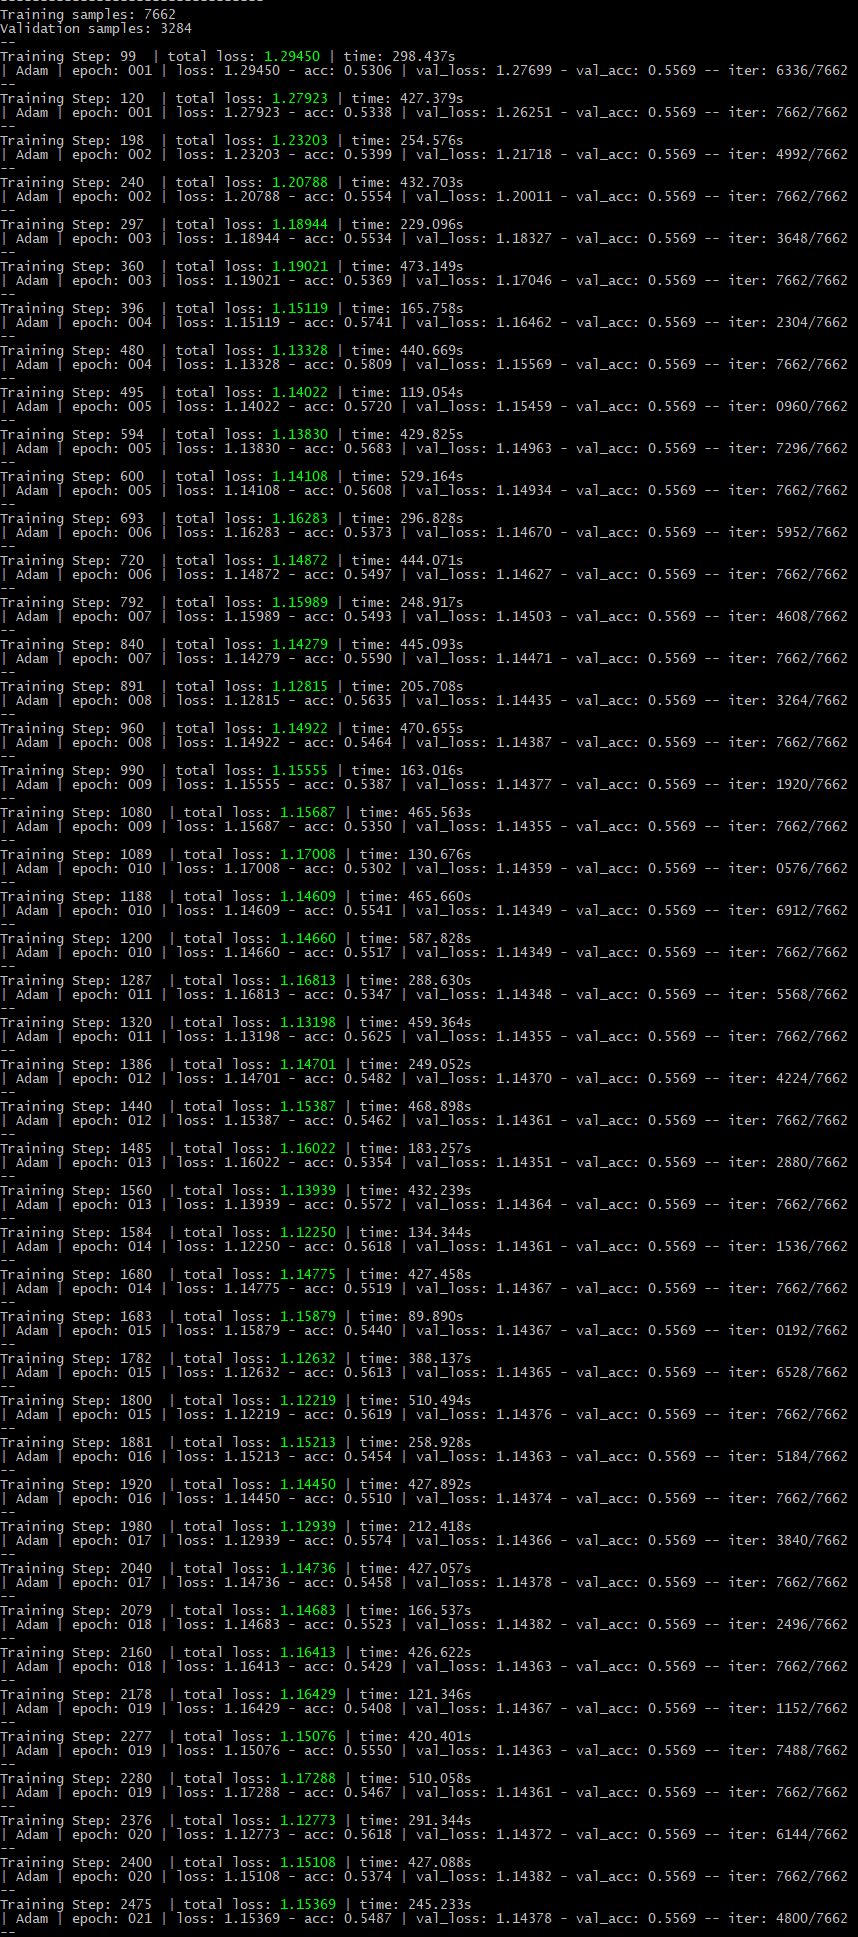
\includegraphics[width=.975\linewidth]{figs/TrainingClas.png}
		\label{fig:NN_C}
	\end{subfigure}
	\begin{subfigure}{.475\textwidth}
		\centering
		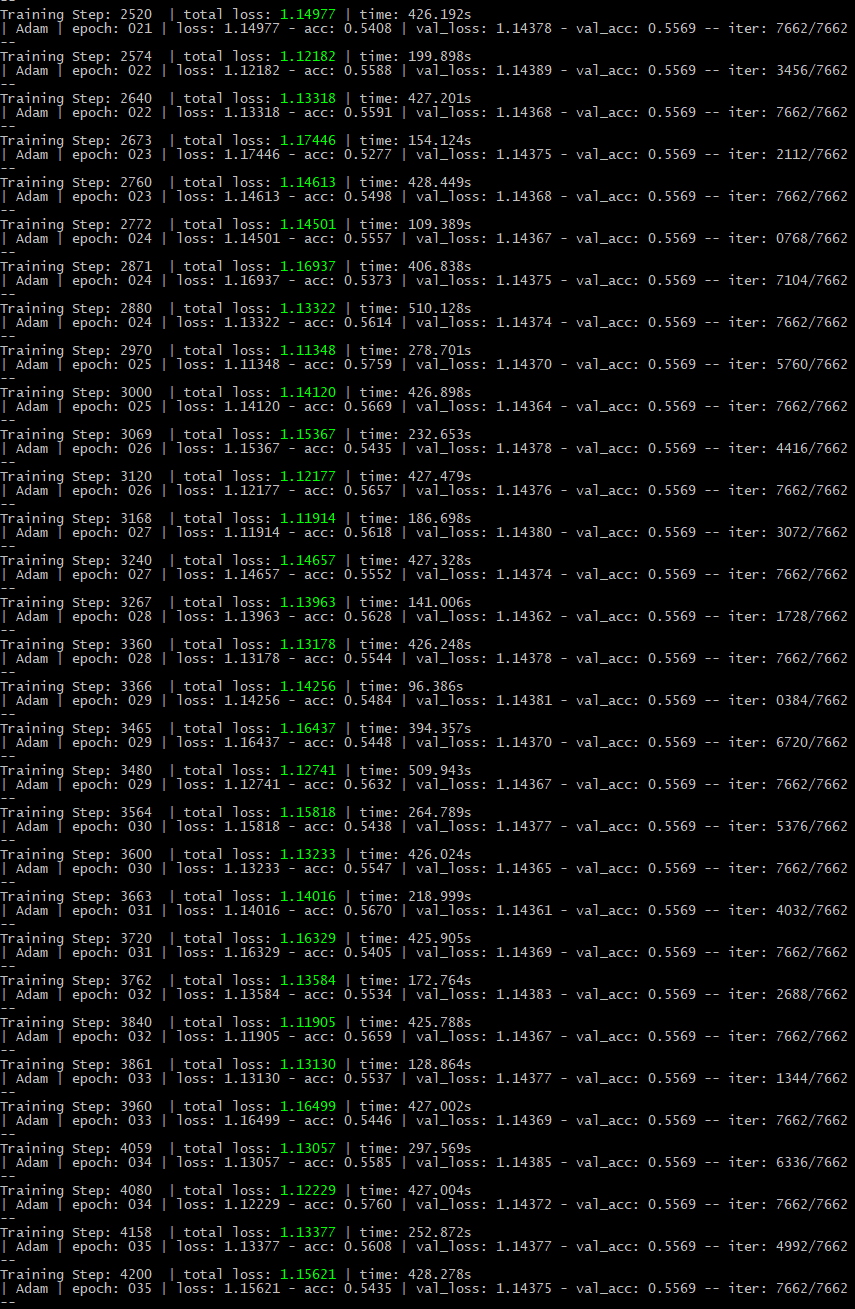
\includegraphics[width=.975\linewidth]{figs/TrainingClas1.png}
		\label{fig:NN_C1}
	\end{subfigure}
	\caption{\footnotesize{Full results training \ac{cnn} with 35 epochs.}}
	\label{fig:an1}
\end{figure}

\section{Results Empirical Approach to Damage Detection} \label{an:coh2}

\begin{table} [H]
	\footnotesize
	\captionsetup{justification=raggedright,singlelinecheck=false}
	\caption{Confusion matrix [Vertical Ground Truth, Horizontal predicted] and F1 classification for interferometry univariate change detection with a threshold of 0.23, 0.31, 0.34. Cohen Kappa Score: 0.05110}
	\begin{tabular}{l|lllll}
            & none  & partial & significant & destroyed & unknown \\\hline
none        & 241.0 & 42.0    & 8.0         & 35.0      & 0.0     \\
partial     & 128.0 & 34.0    & 8.0         & 23.0      & 0.0     \\
significant & 136.0 & 18.0    & 11.0        & 21.0      & 0.0     \\
destroyed   & 91.0  & 14.0    & 7.0         & 23.0      & 0.0     \\
unknown     & 9.0   & 3.0     & 0.0         & 4.0       & 0.0    
	\end{tabular}
	\begin{tabular}{l|llll}
            & precision & recall & f1-score & support \\\hline
none        & 0.22      & 0.17   & 0.19     & 135     \\
partial     & 0.40      & 0.74   & 0.52     & 326     \\
significant & 0.31      & 0.18   & 0.22     & 193     \\
destroyed   & 0.32      & 0.06   & 0.10     & 186     \\
unknown     & 0.00      & 0.00   & 0.00     & 16      \\
avg / total & 0.33      & 0.36   & 0.30     & 856   
	\end{tabular}
	
	\label{tab:matInt2}
\end{table} 

\begin{table} [H]
	\footnotesize
	\captionsetup{justification=raggedright,singlelinecheck=false}
	\caption{Confusion matrix [Vertical Ground Truth, Horizontal predicted] and F1 classification for Hue based univariate change detection with thresholds of 0.08, 0.11, 0.88. Cohen Kappa Score: 0.0543}
	\begin{tabular}{l|lllll}
            & none & partial & significant & destroyed & unknown \\\hline
none        & 79.0 & 41.0    & 205.0       & 1.0       & 0.0     \\
partial     & 31.0 & 28.0    & 132.0       & 2.0       & 0.0     \\
significant & 25.0 & 20.0    & 141.0       & 0.0       & 0.0     \\
destroyed   & 23.0 & 15.0    & 97.0        & 0.0       & 0.0     \\
unknown     & 3.0  & 5.0     & 8.0         & 0.0       & 0.0    
	\end{tabular}
	\begin{tabular}{l|llll}
		& precision & recall & f1-score & support \\ \hline
none        & 0.00 & 0.00 & 0.00 & 135 \\
partial     & 0.49 & 0.24 & 0.32 & 326 \\
significant & 0.26 & 0.15 & 0.19 & 193 \\
destroyed   & 0.24 & 0.76 & 0.37 & 186 \\
unknown     & 0.00 & 0.00 & 0.00 & 16  \\
avg / total & 0.30 & 0.29 & 0.25 & 856\\
	\end{tabular}
	\label{tab:matH2}
\end{table}


\begin{table} [H]
	\footnotesize
	\captionsetup{justification=raggedright,singlelinecheck=false}
	\caption{Confusion matrix [Vertical Ground Truth, Horizontal predicted] and F1 classification for Saturation based univariate change detection with a threshold of 0.08, 0.08, 0.31. Cohen Kappa Score: 0.25029}
	\begin{tabular}{l|lllll}
            & none  & partial & significant & destroyed & unknown \\\hline
none        & 280.0 & 0.0     & 46.0        & 0.0       & 0.0     \\
partial     & 104.0 & 0.0     & 88.0        & 1.0       & 0.0     \\
significant & 53.0  & 0.0     & 133.0       & 0.0       & 0.0     \\
destroyed   & 41.0  & 0.0     & 94.0        & 0.0       & 0.0     \\
unknown     & 6.0   & 0.0     & 10.0        & 0.0       & 0.0   
	\end{tabular}
	\begin{tabular}{l|llll}
            & precision & recall & f1-score & support \\\hline
none        & 0.00      & 0.00   & 0.00     & 135     \\
partial     & 0.58      & 0.86   & 0.69     & 326     \\
significant & 0.00      & 0.00   & 0.00     & 193     \\
destroyed   & 0.36      & 0.72   & 0.48     & 186     \\
unknown     & 0.00      & 0.00   & 0.00     & 16      \\
avg / total & 0.30      & 0.48   & 0.37     & 856     
	\end{tabular}
	
	\label{tab:matS2}
\end{table}

\begin{table} [H]
	\footnotesize
	\captionsetup{justification=raggedright,singlelinecheck=false}
	\caption{Confusion matrix [Vertical Ground Truth, Horizontal predicted] and F1 classification for Value based univariate change detection with a threshold of 0.13, 0.18, 0.26. Cohen Kappa Score: 0.18838}
	\begin{tabular}{l|lllll}
	& none  & partial & significant & destroyed & unknown \\\hline
	none        & 141.0 & 93.0    & 57.0        & 35.0      & 0.0     \\
	partial     & 44.0  & 69.0    & 54.0        & 26.0      & 0.0     \\
	significant & 12.0  & 54.0    & 85.0        & 35.0      & 0.0     \\
	destroyed   & 5.0   & 27.0    & 64.0        & 39.0      & 0.0     \\
	unknown     & 0.0   & 4.0     & 9.0         & 3.0       & 0.0  
	\end{tabular}
	\begin{tabular}{l|llll}
            & precision & recall & f1-score & support \\\hline
none        & 0.28      & 0.29   & 0.29     & 135     \\
partial     & 0.70      & 0.43   & 0.53     & 326     \\
significant & 0.28      & 0.36   & 0.31     & 193     \\
destroyed   & 0.32      & 0.46   & 0.37     & 186     \\
unknown     & 0.00      & 0.00   & 0.00     & 16      \\
avg / total & 0.44      & 0.39   & 0.40     & 856    
	\end{tabular}
	\label{tab:matV2}
\end{table}

\begin{table} [H]
	\footnotesize
	\captionsetup{justification=raggedright,singlelinecheck=false}
	\caption{Confusion matrix [Vertical Ground Truth, Horizontal predicted] and F1 classification for the \ac{cnn} based method. Cohen Kappa Score: 0.0 }	
	\begin{tabular}{l|lllll}
            & none  & partial & significant & destroyed & unknown \\\hline
none        & 101.0 & 33.0    & 6.0         & 186.0     & 0.0     \\
partial     & 41.0  & 24.0    & 5.0         & 123.0     & 0.0     \\
significant & 40.0  & 10.0    & 2.0         & 134.0     & 0.0     \\
destroyed   & 11.0  & 10.0    & 3.0         & 111.0     & 0.0     \\
unknown     & 4.0   & 1.0     & 0.0         & 11.0      & 0.0   
	\end{tabular}
	\begin{tabular}{l|llll}
            & precision & recall & f1-score & support \\\hline
none        & 0.00      & 0.00   & 0.00     & 135     \\
partial     & 0.38      & 1.00   & 0.55     & 326     \\
significant & 0.00      & 0.00   & 0.00     & 193     \\
destroyed   & 0.00      & 0.00   & 0.00     & 186     \\
unknown     & 0.00      & 0.00   & 0.00     & 16      \\
avg / total & 0.15      & 0.38   & 0.21     & 856  
	\end{tabular}
	\label{tab:matCNN2}
\end{table}

\begin{table} [H]
	\footnotesize
	\captionsetup{justification=raggedright,singlelinecheck=false}
	\caption{Confusion matrix [Vertical Ground Truth, Horizontal predicted] and F1 classification for the Copernicus classification. Cohen Kappa Score: 0.07871 }
	\begin{tabular}{l|lllll}		
		& none  & partial & significant & destroyed & unknown \\\hline
none        & 101.0 & 33.0    & 6.0         & 186.0     & 0.0     \\
partial     & 41.0  & 24.0    & 5.0         & 123.0     & 0.0     \\
significant & 40.0  & 10.0    & 2.0         & 134.0     & 0.0     \\
destroyed   & 11.0  & 10.0    & 3.0         & 111.0     & 0.0     \\
unknown     & 4.0   & 1.0     & 0.0         & 11.0      & 0.0    
	\end{tabular}
	\begin{tabular}{l|llll}
            & precision & recall & f1-score & support \\\hline
none        & 0.20      & 0.82   & 0.32     & 135     \\
partial     & 0.51      & 0.31   & 0.39     & 326     \\
significant & 0.31      & 0.12   & 0.18     & 193     \\
destroyed   & 0.12      & 0.01   & 0.02     & 186     \\
unknown     & 0.00      & 0.00   & 0.00     & 16      \\
avg / total & 0.32      & 0.28   & 0.24     & 856  \\  
	\end{tabular}
	\label{tab:matCop2}
\end{table}
